
\section{Results}

\begin{table*}
    \centering
    \begin{adjustbox}{max width=\textwidth}
        \begin{tabular}{|c|c|c|c|c|c|c|c|c|c|c|c|c|c|c|}
            \hline
            \multirow{3}{*}{Model}     &         & Average  & Joint    & Average        & Joint          &                & \multirow{2}{*}{Intent}   & Requested & \multirow{2}{*}{Response} & \multirow{2}{*}{Response} &         & Average    & Joint      &          \\
                                       & Setting & Action   & Action   & Goal           & Goal           & Inform         & \multirow{2}{*}{Accuracy} & Slots     & \multirow{2}{*}{GLEU}     & \multirow{2}{*}{ROUGE-2}  & Success & UserAction & UserAction & Combined \\
                                       &         & Accuracy & Accuracy & Accurracy      & Accuracy       &                &                           & F1        &                           &                           &         & Accuracy   & Accuracy   &          \\ \hline
            \multirow{3}{*}{SimpleTOD} & all     & 49.08    & 37.66    & 47.85          & 24.18          & 55.65          & 78.60                     & 94.08     & 20.64                     & 27.68                     & 47.27   & 66.42      & 57.46      & 72.10    \\
                                       & seen    & 51.43    & 40.26    & 52.00          & 29.35          & 58.35          & 80.07                     & 94.55     & 24.89                     & 27.68                     & 50.13   & 68.88      & 60.31      & 79.13    \\
                                       & unseen  & 48.29    & 37.12    & 46.27          & 22.72          & 54.28          & 78.63                     & 93.92     & 19.24                     & 27.68                     & 46.17   & 65.55      & 56.65      & 69.47    \\ \hline
            {SimpleTOD w/}             & all     & 55.18    & 43.42    & 58.03          & 30.36          & 68.30          & 82.34                     & 95.72     & 22.03                     & 21.88                     & 60.47   & 70.30      & 60.23      & 86.41    \\
            {Schema \&}                & seen    & 57.28    & 46.01    & 61.29          & 34.88          & 70.05          & 83.32                     & 96.05     & 25.68                     & 21.88                     & 62.68   & 72.34      & 62.61      & 92.04    \\
            {DB Results}               & unseen  & 54.64    & 42.85    & 57.35          & 29.20          & 68.10          & 82.19                     & 95.71     & 20.40                     & 21.88                     & 60.48   & 70.19      & 60.24      & 84.69    \\ \hline
            \multirow{3}{*}{Our}       & all     & 58.32    & 46.31    & \textbf{72.38} & \textbf{48.44} & \textbf{73.08} & 84.83                     & 95.53     & 20.04                     & 22.26                     & 62.19   & 73.20      & 64.20      & 87.67    \\
                                       & seen    & 60.19    & 48.69    & \textbf{74.23} & \textbf{52.05} & \textbf{74.72} & 85.48                     & 95.88     & 24.66                     & 22.26                     & 63.85   & 74.89      & 66.24      & 93.95    \\
                                       & unseen  & 57.42    & 45.21    & \textbf{72.03} & \textbf{47.83} & \textbf{71.68} & 84.45                     & 95.42     & 18.51                     & 22.26                     & 61.63   & 72.56      & 63.46      & 85.16    \\ \hline
        \end{tabular}
    \end{adjustbox}
    \caption{Main Results. For end-to-end systems, our approach outperforms existing baselines across all metrics, particularly there is significant improvement in key metrics like Average/Joint Goal Accuracy and Inform.}
    \label{tab:main-results}
\end{table*}

\begin{table}
    \begin{adjustbox}{max width=0.45\textwidth}
        \begin{tabular}{|c|c|c|c|c|}
            \hline
            \multirow{2}{*}{Model} & Intent   & Requested & Average & Joint \\
                                   & Accuracy & Slot F1   & GA      & GA    \\ \hline
            SGD Baseline           & 90.60    & 96.50     & 56      & 25.40 \\ \hline
            FastSGT                & 90.33    & 96.33     & 60.66   & 29.20 \\ \hline
            Seq2Seq-DU             & 91.00    & -         & -       & 30.10 \\ \hline
            DSGFNET                & -        & -         & -       & 32.10 \\ \hline
            Ours                   & 81.49    & 95.97     & 74.08   & 49.73 \\ \hline
        \end{tabular}
    \end{adjustbox}
    \caption{Results on SGD test set. Our approach significantly outperforms baselines methods in terms of average and joint goal accuracy.}
    \label{tab:other-results}
\end{table}

Since there are no end-to-end TOD systems for the SGD dataset, we re-implemented some of the popular baseline methods to
compare with our approach and present the results in Table~\ref{tab:main-results}. We can see that our model outperforms all the
baselines methods across all metrics.

We evaluate the DST performance of our model with the evaluation script provided by the SGD dataset and present our results along
with other baseline DST models in Table~\ref{tab:other-results}.
We can see that even though our method is not specifically designed for DST, still it significantly outperforms the baselines models in the
important metrics: Average and Joint Goal Accuracy.

\subsection{Long Range Dependency}

\begin{figure}
    \centering
    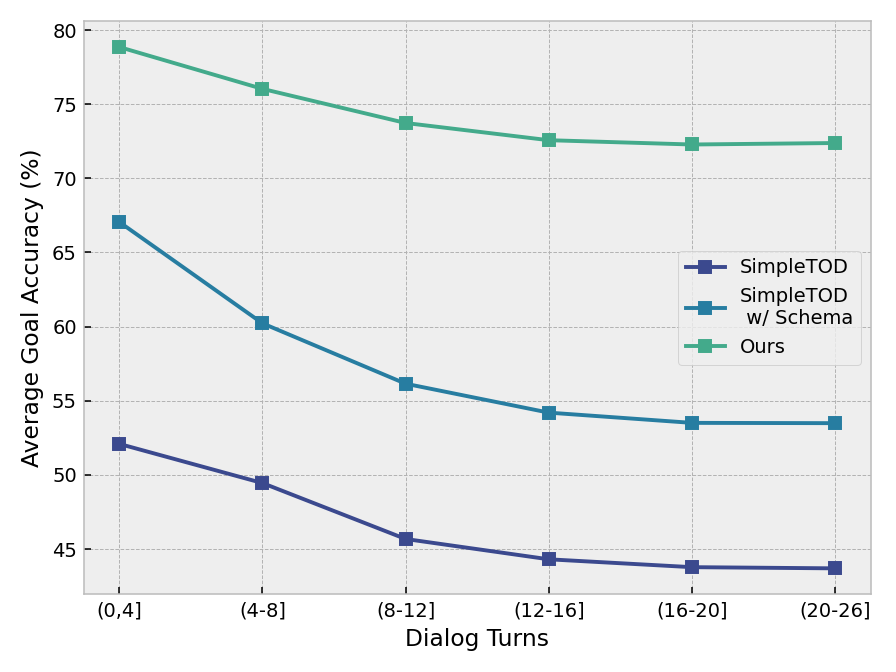
\includegraphics[width=\linewidth]{assets/dialog_turns.png}
    \caption{
        Performance of dialog systems on the SGD test set with respect to dialog turns
    }
    \label{fig:dialog_turns}
\end{figure}

In order to process dialogs that have a large number of turns, a system must be effective at capturing long range dependencies.
To test this ability, we group the test dialogs based on the number of turns and evaluate the performance of our model and a few baseline models on each group~\cite{sun2022mars}.
As shown in Figure~\ref{fig:dialog_turns}, our model outperforms the baseline models on all groups. Upon careful inspection, one can see that
the performance of the baselines models decrease sharply for the first few groups when compared to our model. However, for dialogs with more than 12 turns,
the performance of all models degrade in a similar pattern.

To understand how well our model can handle long range dependencies in dialogs, we group the test dialogs based on the number of turns and
evaluate the performance of our model on each group~\cite{sun2022mars}.
we compare the performance of our model with the baseline model on the SGD test set.


\subsection{Ablation Study}

To get a better understanding of the different components of our model, we report an ablation study in Table \ref{tab:ablation-results}.
We can see that removing list of system actions and user actions has decreased the metrics related to system actions the most: AAA, JAA, Inform and Success,
but there is no significant decrease in metrics related to DST and system response. User actions and service results have some correlation with DST,
so these components have a larger effect on DST when compared to list of system actions. As expected, the major drop in performance occurs when we
elect to drop schema. Not only does the performance drops significantly in the unseen domain, there is also a performance degradation
across all other metrics by a noticeable amount. This shows that schema is an important component in our approach as
it not only helps the model to generalize to new domains, but also plays a crucial role in the overall performance of the system.
The last row in the table shows how important the two step training process is for our model, as we can see that there is a significant
drop in performance of our model without it.

\begin{table*}
    \centering
    \begin{adjustbox}{max width=\textwidth}
        \begin{tabular}{|c|c|c|c|c|c|c|c|c|c|c|c|c|}
            \hline
            \multirow{3}{*}{Model} &         & Average  & Joint    & Average        & Joint          &                & \multirow{2}{*}{Intent}   & Requested & \multirow{2}{*}{Response} & \multirow{2}{*}{Response} &         &          \\
                                   & Setting & Action   & Action   & Goal           & Goal           & Inform         & \multirow{2}{*}{Accuracy} & Slots     & \multirow{2}{*}{GLEU}     & \multirow{2}{*}{ROUGE-2}  & Success & Combined \\
                                   &         & Accuracy & Accuracy & Accurracy      & Accuracy       &                &                           & F1        &                           &                           &         &          \\ \hline
            \multirow{3}{*}{Our}   & all     & 58.32    & 46.31    & \textbf{72.38} & \textbf{48.44} & \textbf{73.08} & 84.83                     & 95.53     & 20.04                     & 22.26                     & 62.19   & 87.67    \\
                                   & seen    & 60.19    & 48.69    & \textbf{74.23} & \textbf{52.05} & \textbf{74.72} & 85.48                     & 95.88     & 24.66                     & 22.26                     & 63.85   & 93.95    \\
                                   & unseen  & 57.42    & 45.21    & \textbf{72.03} & \textbf{47.83} & \textbf{71.68} & 84.45                     & 95.42     & 18.51                     & 22.26                     & 61.63   & 85.16    \\ \hline
            {w/o}                  & all     & 57.34    & 45.26    & 71.51          & 42.68          & 64.15          & 88.22                     & 95.72     & 20.70                     & 23.81                     & 60.98   & 83.27    \\
            {User}                 & seen    & 59.48    & 47.83    & 73.86          & 47.02          & 65.80          & 89.02                     & 96.07     & 25.96                     & 23.81                     & 63.17   & 90.44    \\
            {Actions}              & unseen  & 56.46    & 44.41    & 71.05          & 41.78          & 63.09          & 87.94                     & 95.59     & 18.82                     & 23.81                     & 60.73   & 80.73    \\ \hline
            {w/o Sys}              & all     & 57.98    & 45.86    & 72.86          & 44.52          & 60.13          & 87.56                     & 96.00     & 21.02                     & 24.94                     & 61.91   & 82.04    \\
            {Action}               & seen    & 60.12    & 48.37    & 75.11          & 48.77          & 61.69          & 88.25                     & 96.32     & 26.56                     & 24.94                     & 64.04   & 89.43    \\
            {Names}                & unseen  & 57.29    & 45.26    & 72.44          & 43.60          & 59.61          & 87.38                     & 95.91     & 19.16                     & 24.94                     & 61.75   & 79.84    \\ \hline
            {w/o}                  & all     & 53.67    & 41.73    & 71.54          & 43.20          & 50.96          & 87.50                     & 95.48     & 17.62                     & 23.90                     & 56.89   & 71.54    \\
            {DB}                   & seen    & 55.73    & 43.91    & 73.87          & 47.62          & 53.03          & 88.26                     & 95.85     & 23.12                     & 23.90                     & 59.08   & 79.17    \\
            {Results}              & unseen  & 53.17    & 41.52    & 71.04          & 42.17          & 50.33          & 87.19                     & 95.36     & 16.07                     & 23.90                     & 56.95   & 69.70    \\ \hline
            {w/o}                  & all     & 54.14    & 43.07    & 64.70          & 38.47          & 59.88          & 83.14                     & 94.67     & 21.15                     & 22.66                     & 53.88   & 78.03    \\
            {Domain}               & seen    & 56.61    & 45.92    & 67.62          & 43.39          & 62.30          & 84.34                     & 95.10     & 27.10                     & 22.66                     & 56.64   & 86.57    \\
            {Schema}               & unseen  & 53.22    & 42.20    & 63.95          & 37.59          & 58.65          & 82.96                     & 94.52     & 19.33                     & 22.66                     & 53.25   & 75.28    \\ \hline
            {w/o}                  & all     & 40.38    & 30.71    & 62.47          & 39.52          & 48.13          & 75.08                     & 92.80     & 11.41                     & 23.21                     & 44.27   & 57.61    \\
            {Two Step}             & seen    & 41.96    & 32.42    & 64.66          & 42.76          & 50.26          & 75.75                     & 93.13     & 13.75                     & 23.21                     & 46.47   & 62.11    \\
            {Training}             & unseen  & 40.25    & 30.66    & 62.60          & 39.25          & 47.55          & 75.79                     & 92.90     & 11.03                     & 23.21                     & 44.32   & 56.97    \\ \hline
        \end{tabular}
    \end{adjustbox}
    \caption{Ablation Study of our model.}
    \label{tab:ablation-results}
\end{table*}




\subsection{SGD-x}
\textbf{I could show SGD results for each domain and compare them with 2 other papers as they have reported these results as well}

\textbf{I have ablation results of 2 step training for SimpleTod and SimpleTOD w/ schema. How should I add them?}

\textbf{Add a graph similar to that in sgd-x paper with JGA for SGD-x for our model and SimpleTOD w/ schema. }



